\documentclass[12pt, tikz, border=5mm]{standalone}
\usepackage{tikz}
\usetikzlibrary{intersections}
\begin{document}
 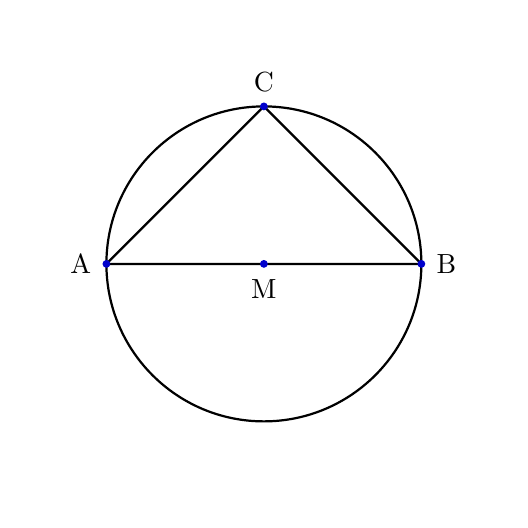
\begin{tikzpicture}[thick]
% %Zeichenbereich beschneiden
% \clip(0,0)coordinate(M)circle[radius=6cm];
% %Umkreis zeichnen
% \draw[name path=k1] (M) circle [radius=5.5cm];
% %Punkt B festlegen
% \coordinate(B)at(5.5,0);
% %Konstruktion Punkt C
% \path[name path=k2](B)circle[radius=8cm];%
% \path[name intersections={of=k1 and k2,name=C}];
% %Konstruktion Punkt A
% \path[name path=g](C-2)--(B)--([turn]0:35);
% \path[name intersections={of=k1 and g,name=A}];
% % Dreieck zeichnen
% \draw(A-2)--(B)--(C-1)--cycle;
\newcommand{\radius}{2}

%Zeichenbereich beschneiden
\clip(0,0)coordinate(M)circle[radius=\radius+1];


%Umkreis zeichnen
\draw[] (M) circle [radius=\radius];


% %Punkt  festlegen
 \coordinate(B)at(\radius,0);
 \coordinate(A)at(-\radius,0);
\coordinate(C)at(0,\radius);
% %Konstruktion Punkt C
 \draw (A) -- (B) -- (C) -- cycle;
%Punkte einzeichnen und beschriften
 \foreach \p/\b/\o in {A/A/left,B/B/right,C/C/above,M/M/below}
   \node[fill=blue!80!black,circle,inner sep=1pt,label=\o:\b] at (\p){};


\end{tikzpicture}
\end{document}